\section{Results}

We report the main cohort comparison first, then the mechanism-focused
ablations, and finally the harder-task check.

\subsection{Main Contract x Runtime Effect}

The main effect is a stable qualitative ordering across navigation easy,
tabletop manipulation easy, harder navigation, and harder manipulation. In
each slice, P0/R0 is the weakest cell. Pairing the same under-specified
contract with R1 changes the outcome: P0/R1 succeeds where P0/R0 fails, while
P1/R0, P1/R1, P2/R0, and P2/R1 remain strong. The same ordering holds
across both task families and persists as tasks become harder. Because the
planner backend and exposed task executors are deterministic by design, each
cell is interpreted as a descriptive comparison over a fixed cohort of task
instances rather than as an estimate from repeated stochastic rollouts.

\begin{figure*}[t]
  \centering
  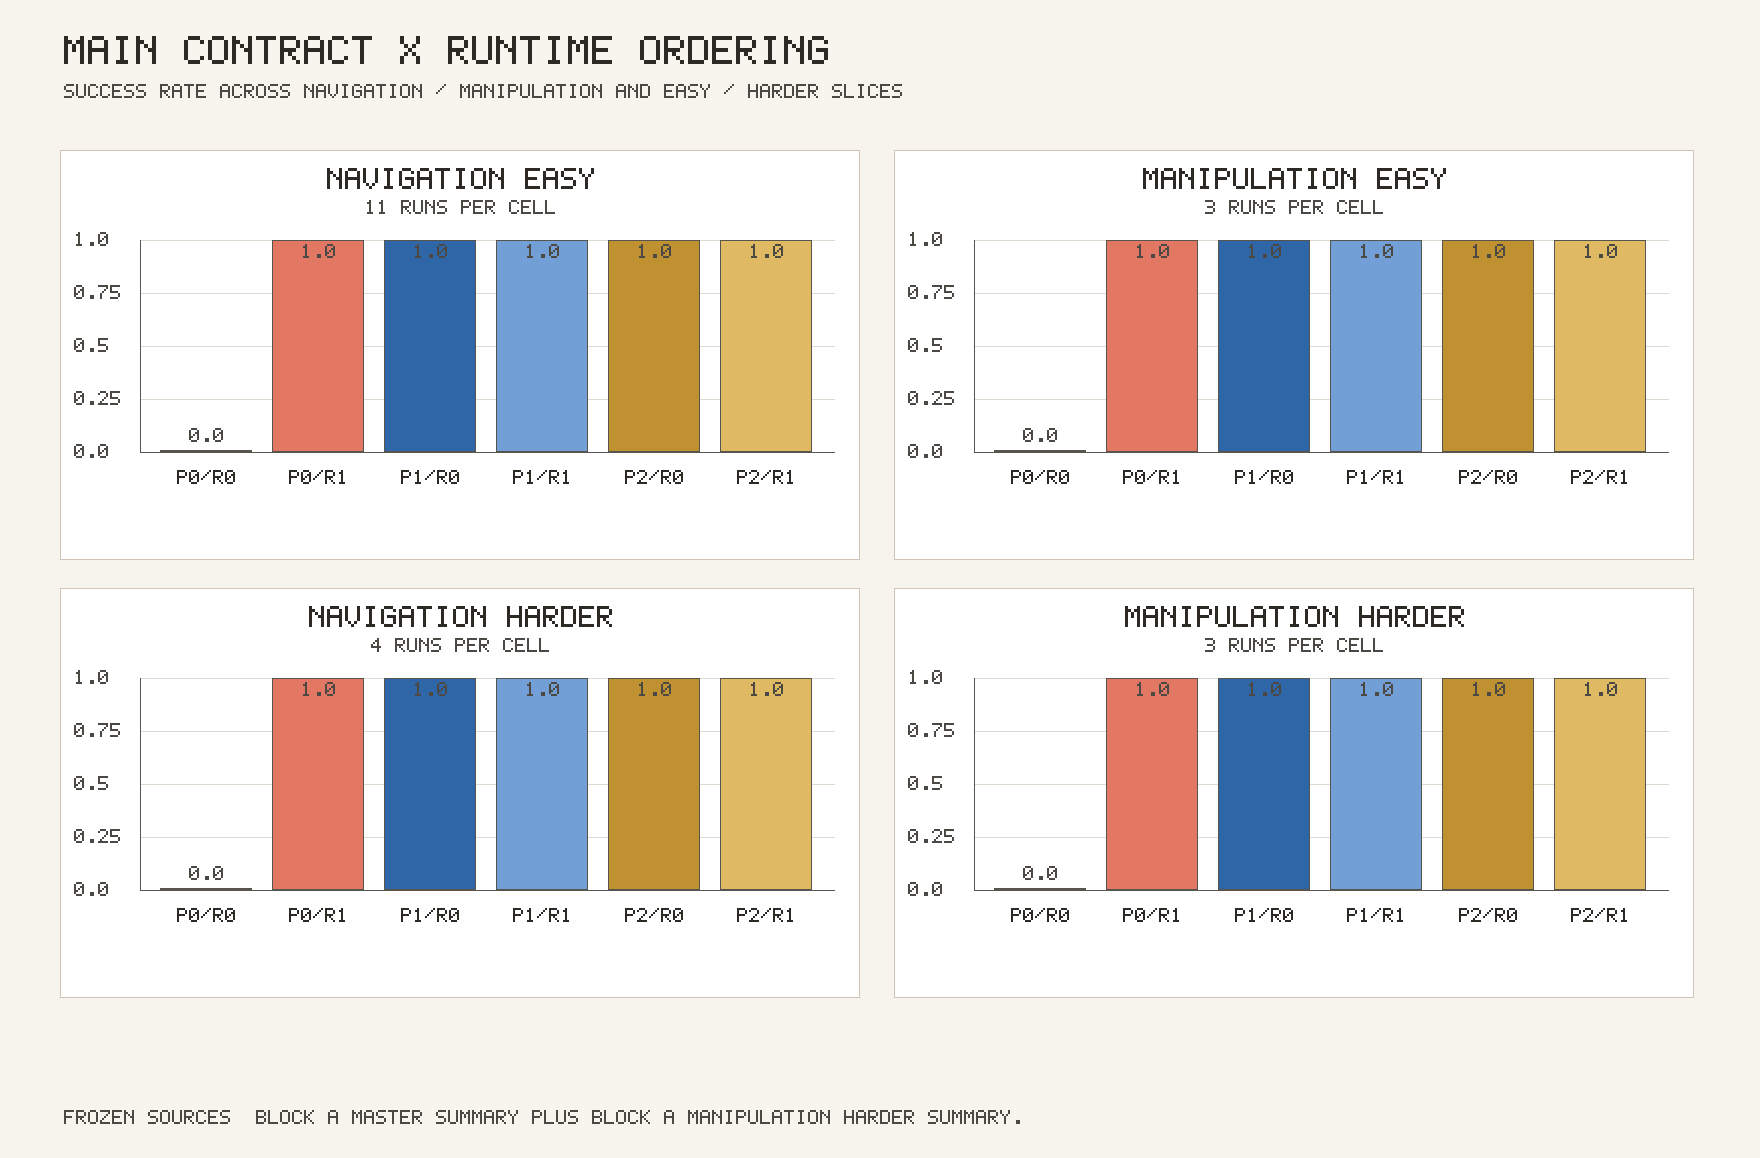
\includegraphics[width=\textwidth]{figures/main_condition_ordering.png}
  \caption{Success rate for the retained contract and runtime conditions across both task families and both difficulty slices. The under-specified direct-action contract \texttt{P0/R0} is the weakest cell, \texttt{P0/R1} recovers, and the typed tool-call contracts remain successful in the covered easy and harder slices.}
  \label{fig:main-condition-ordering}
\end{figure*}

\begin{table*}[!t]
  \centering
  \caption{Outcome summary across the four main cohorts. Each entry keeps success, invalid/run, and retry/run together so the table still distinguishes recovered \texttt{P0/R1} cells from clean structured cells.}
  \label{tab:main-outcome-summary}
  \footnotesize
  \setlength{\tabcolsep}{5pt}
  \rowcolors{2}{ralPanel}{white}
  \begin{tabularx}{\textwidth}{L{1.1cm} Y Y Y Y}
    \toprule
    Cell & \thead{Navigation\\Easy} & \thead{Manipulation\\Easy} & \thead{Navigation\\Harder} & \thead{Manipulation\\Harder} \\
    \midrule
    P0/R0 & 0/11; 1.0; 0.0 \scriptsize[fail] & 0/3; 1.0; 0.0 \scriptsize[fail] & 0/4; 1.0; 0.0 \scriptsize[fail] & 0/3; 1.0; 0.0 \scriptsize[fail] \\
    P0/R1 & 11/11; 1.0; 1.0 \scriptsize[recov.] & 3/3; 1.0; 1.0 \scriptsize[recov.] & 4/4; 1.0; 1.0 \scriptsize[recov.] & 3/3; 1.0; 1.0 \scriptsize[recov.] \\
    P1/R0 & 11/11; 0.0; 0.0 \scriptsize[clean] & 3/3; 0.0; 0.0 \scriptsize[clean] & 4/4; 0.0; 0.0 \scriptsize[clean] & 3/3; 0.0; 0.0 \scriptsize[clean] \\
    P1/R1 & 11/11; 0.0; 0.0 \scriptsize[clean] & 3/3; 0.0; 0.0 \scriptsize[clean] & 4/4; 0.0; 0.0 \scriptsize[clean] & 3/3; 0.0; 0.0 \scriptsize[clean] \\
    P2/R0 & 11/11; 0.0; 0.0 \scriptsize[clean] & 3/3; 0.0; 0.0 \scriptsize[clean] & 4/4; 0.0; 0.0 \scriptsize[clean] & 3/3; 0.0; 0.0 \scriptsize[clean] \\
    P2/R1 & 11/11; 0.0; 0.0 \scriptsize[clean] & 3/3; 0.0; 0.0 \scriptsize[clean] & 4/4; 0.0; 0.0 \scriptsize[clean] & 3/3; 0.0; 0.0 \scriptsize[clean] \\
    \bottomrule
  \end{tabularx}
  \\[1pt]
  {\raggedright\scriptsize Cell entries are \emph{success; invalid/run; retry/run} followed by overall status: [fail] = no runs succeeded, [recov.] = all succeeded via runtime recovery, [clean] = all succeeded without recovery.\par}
\end{table*}


Table~\ref{tab:main-outcome-summary} records the same four evaluation cohorts
in a compact layout that keeps success, invalid-action exposure, and
retries readable without forcing planner/tool counts into every cell.
Figure~\ref{fig:main-condition-ordering} makes the same distinction visually:
the recovered \texttt{P0/R1} cells are separated from the clean
\texttt{P1}/\texttt{P2} cells, and the cell text carries the status label so
that the comparison does not rely on color alone.

The same comparison separates the roles of contract design and runtime
validation. Invalid-action failures are concentrated in the P0 cells, showing
that loose task-level verbs are brittle at the planner/executor boundary. Once
the planner is forced into a typed tool namespace, the dominant failure mode
disappears in the evaluated fixed-R0 ablation. Within the successful
structured conditions, P2 matches P1 on success while showing lower
planner/tool overhead across the evaluated \texttt{P1} versus \texttt{P2}
comparisons.
Table~\ref{tab:planner-tool-overhead-summary} isolates that workload
comparison so the manuscript can report it without overloading the outcome
table. Figure~\ref{fig:planner-tool-overhead} compresses those
comparisons into one workload mark per row because planner and tool counts are
equal within the plotted \texttt{P1}/\texttt{P2} pairs. We interpret that
pattern as a workload association within already-strong contracts, not as
evidence of a separate success mechanism.

\begin{figure*}[t]
  \centering
  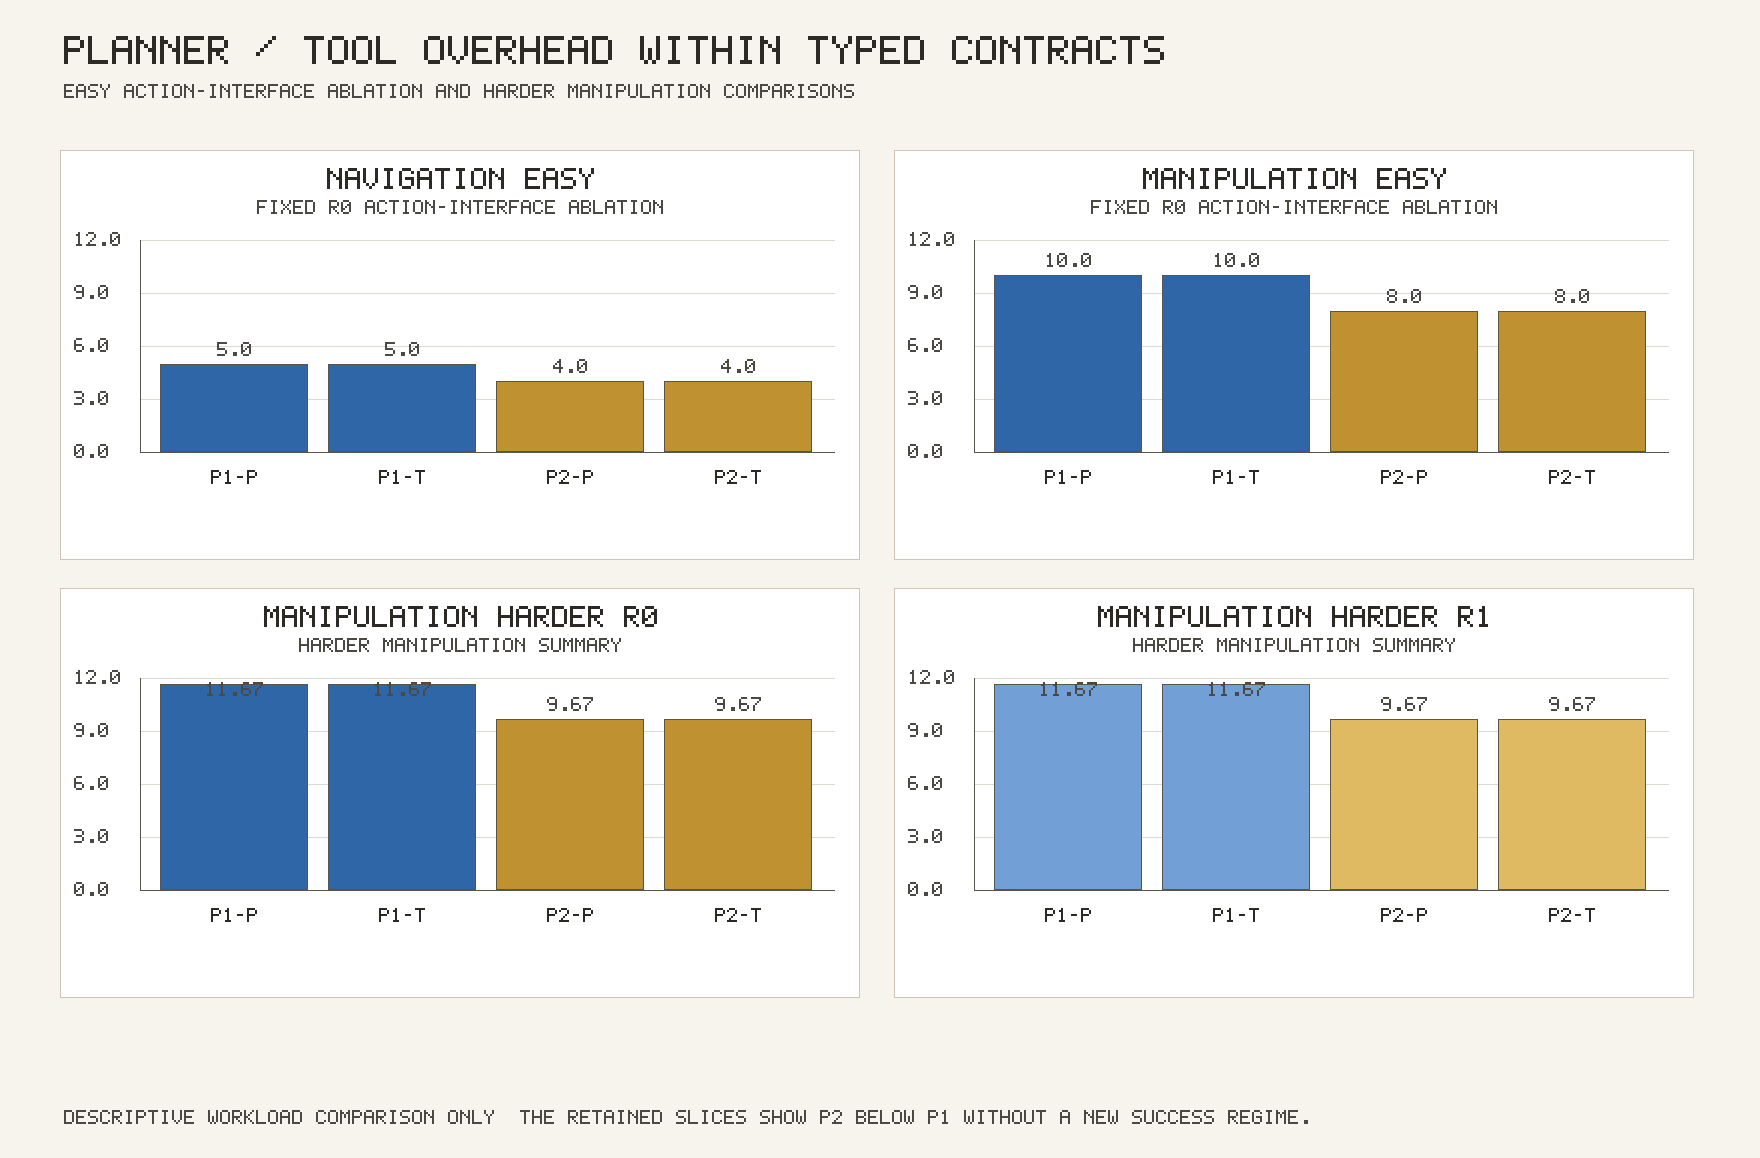
\includegraphics[width=\textwidth]{figures/planner_tool_overhead.png}
  \caption{Planner and tool calls in the retained \texttt{P1} versus \texttt{P2} comparisons. In the easy fixed-\texttt{R0} action-interface ablation and in the harder manipulation slice, \texttt{P2} keeps the same success profile as \texttt{P1} while using fewer planner/tool calls. This is a descriptive slice-level comparison, not a broader statistical claim.}
  \label{fig:planner-tool-overhead}
\end{figure*}


\begin{table*}[!t]
  \centering
  \caption{Planner/tool workload across the four main cohorts. Figure~\ref{fig:planner-tool-overhead} compresses the duplicated plotted pairs for readability; this table preserves the full per-cell breakdown.}
  \label{tab:planner-tool-overhead-summary}
  \footnotesize
  \setlength{\tabcolsep}{5pt}
  \rowcolors{2}{ralPanel}{white}
  \begin{tabularx}{\textwidth}{L{1.1cm} Y Y Y Y Y}
    \toprule
    Cell & \thead{Navigation\\Easy} & \thead{Manipulation\\Easy} & \thead{Navigation\\Harder} & \thead{Manipulation\\Harder} & \thead{$\Delta$ vs P1\\(tool calls)} \\
    \midrule
    P0/R0\textsuperscript{$\dagger$} & 1.0/0.0 & 1.0/0.0 & 1.0/0.0 & 1.0/0.0 & --- \\
    P0/R1 & 3.82/2.82 & 9.0/8.0 & 6.75/5.75 & 10.67/9.67 & --- \\
    P1/R0 & 4.82/4.82 & 10.0/10.0 & 7.75/7.75 & 11.67/11.67 & 0 \\
    P1/R1 & 4.82/4.82 & 10.0/10.0 & 7.75/7.75 & 11.67/11.67 & 0 \\
    P2/R0 & 3.82/3.82 & 8.0/8.0 & 6.75/6.75 & 9.67/9.67 & $-$1.0 to $-$2.0 \\
    P2/R1 & 3.82/3.82 & 8.0/8.0 & 6.75/6.75 & 9.67/9.67 & $-$1.0 to $-$2.0 \\
    \bottomrule
  \end{tabularx}
  \\[1pt]
  {\raggedright\scriptsize Cell entries are \emph{planner calls/tool calls per run}. The $\Delta$ column shows the per-cohort range of P2 savings relative to P1.\\
  $\dagger$ P0/R0 reports 0.0 tool calls because all runs fail at the planner stage (invalid action); no tool is dispatched.\par}
\end{table*}


\subsection{Action-Interface and Runtime-Only Ablations}

The targeted ablations use different easy-task subsets: the runtime-only slice
deliberately includes recoverable invalid-first-action probes under fixed P1,
whereas the action-interface ablation uses clean easy tasks under fixed R0.
Together they isolate the two design axes within the same execution-design
framing.

With the contract fixed at P1, moving from R0 to R1 raises success from
2/4 to 4/4 across two navigation tasks and two tabletop manipulation tasks.
The mechanism is recovery, not suppression: invalid-action runs remain 2
under both runtimes, but successful invalid-action recoveries rise from 0 to
2 once validation and one retry are enabled. The same direction appears in
each family separately, with navigation and manipulation each moving from
0.5 to 1.0 success in this slice. In the runtime traces, the first retry for
the navigation probe switches from \texttt{move\_to\_goal} to
\texttt{get\_robot\_state}, and the first retry for the manipulation probe
switches from \texttt{move\_object} to \texttt{get\_object\_state}; the repair
signal is the explicit error string rather than a new second-pass tool schema.

With runtime fixed at R0, P0/R0 fails on all 4/4 evaluated tasks and
accumulates four total invalid actions, whereas P1/R0 and P2/R0 succeed on
all 4/4 tasks and reduce invalid actions to zero. This establishes an
independent contract effect: once the planner must emit dispatchable tool
calls, the invalid-action failures that dominate the under-specified interface
disappear in this slice. The same comparison also shows the narrower P2
effect: P1/R0 and P2/R0 have the same success profile, but average planner
and tool calls each fall from roughly 7.5 to 6.0.

\begin{figure*}[t]
  \centering
  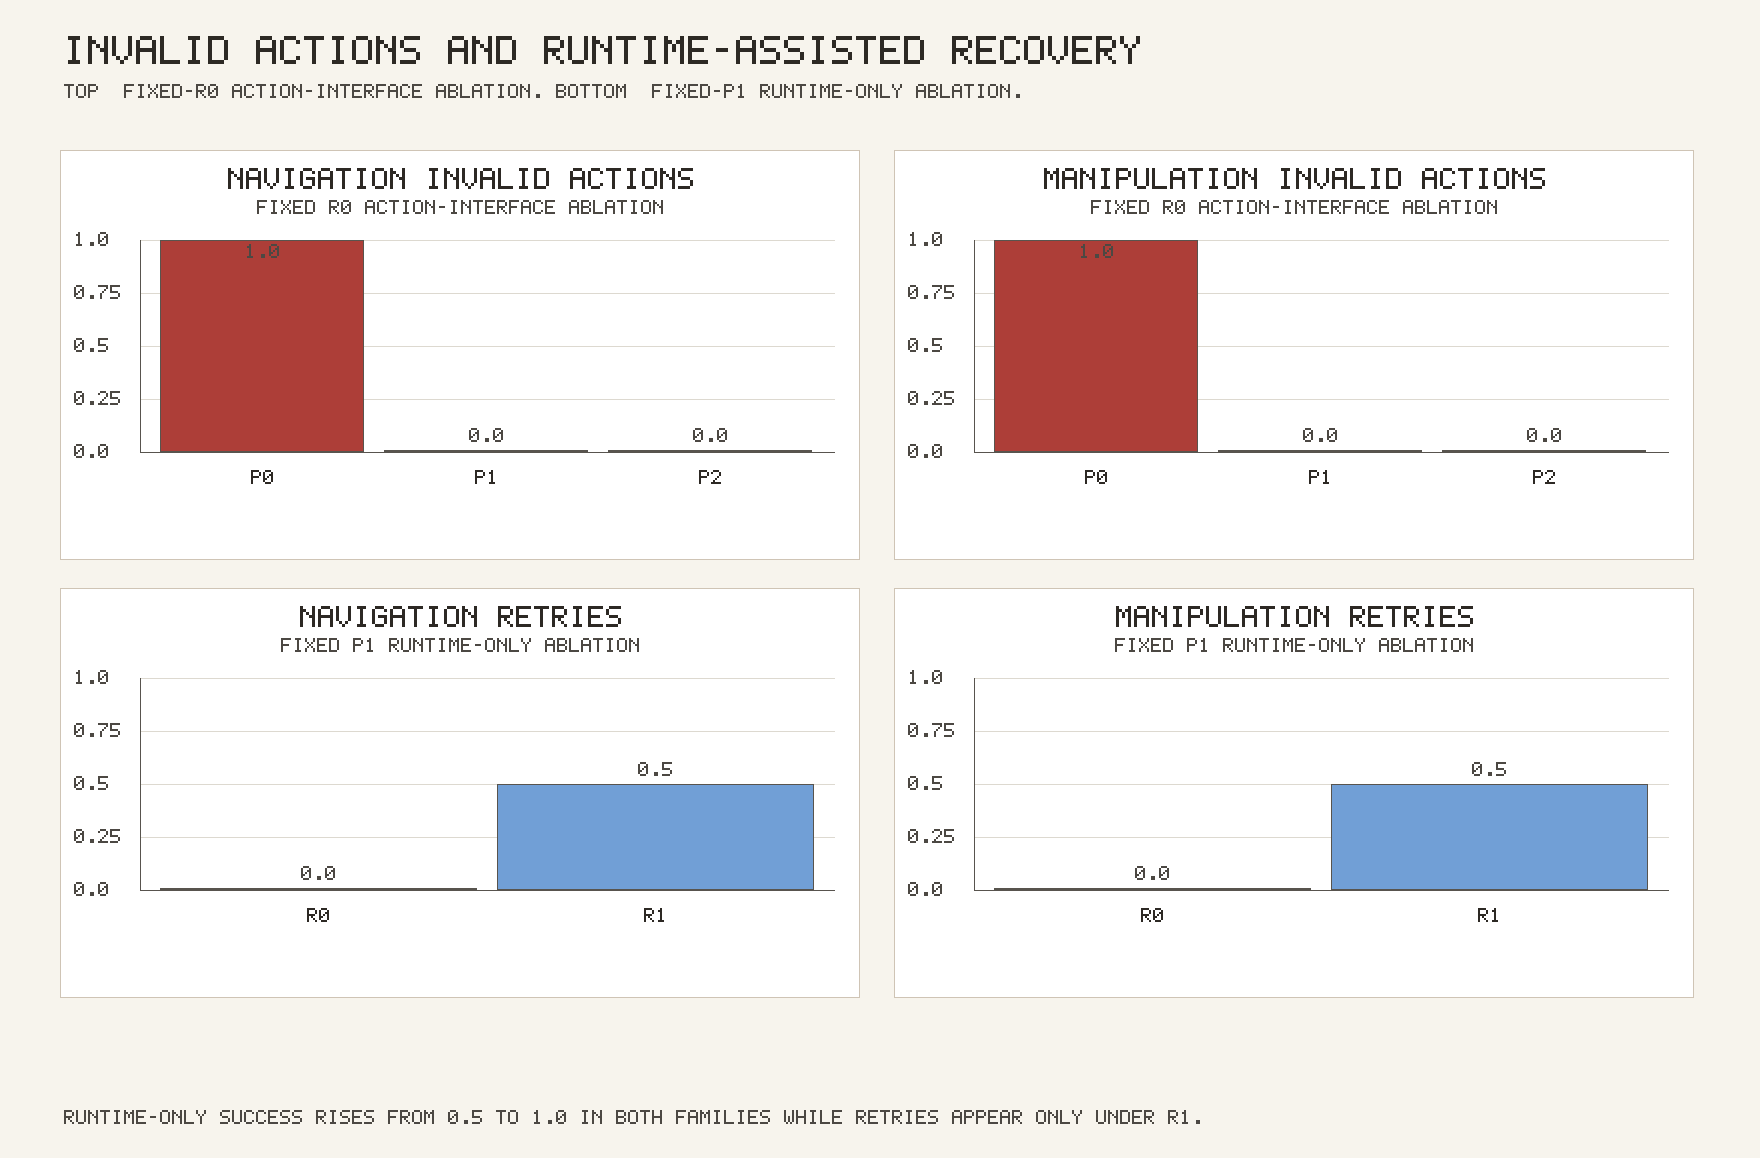
\includegraphics[width=\textwidth]{figures/invalid_actions_recovery.png}
  \caption{Top: under fixed \texttt{R0}, typed tool-call contracts remove invalid actions in both families. Bottom: under fixed \texttt{P1}, validate-and-retry \texttt{R1} adds retries only on recoverable invalid-first-action probes and raises success from 0.5 to 1.0 in both families.}
  \label{fig:invalid-actions-recovery}
\end{figure*}


Figure~\ref{fig:invalid-actions-recovery} makes both mechanisms visible in one
place: the fixed-R0 panel shows typed contracts eliminating invalid actions,
while the fixed-P1 runtime panel shows R1 converting the invalid half of the
runtime-only slice from failure into recovery, with retries rising from 0.0 to
0.5 per run.

The failure traces identify the dominant P0 failure mode. In navigation, failing
P0 runs repeatedly emit the unsupported tool name
\texttt{move\_to\_goal}; in tabletop manipulation, they emit
\texttt{move\_object}. Both are semantically plausible task verbs, but the
executor accepts \texttt{navigate\_to} and
\texttt{scripted\_pick\_place\_step} instead. R1 helps because the runtime
parses the JSON, checks the proposed tool against the exposed task namespace,
enforces the required argument set, and then returns the literal validation
error string to the planner before one retry. The retry does not expose a
stronger second schema than P1: the same tool list and required arguments were
already available on the first pass. Instead, it turns a terminating handoff
failure into a recoverable one by appending a concrete error such as
\texttt{unknown tool: move\_to\_goal} or
\texttt{unknown tool: move\_object} to the repair instruction.
Figure~\ref{fig:system-overview} includes compact navigation and manipulation
traces for exactly that
non-dispatchable-to-corrected transition.

\subsection{Harder-Task Robustness}

The harder-task slices increase planner/tool overhead without changing the
condition ordering. In harder navigation, the easy-slice ranking is preserved,
while successful cells require roughly three additional planner or tool calls
per run. In harder tabletop manipulation, P0/R0 fails on all 3/3 tasks,
P0/R1 recovers all 3/3 with one retry per task, and P1/P2 remain fully
successful under both runtimes.

The P1 versus P2 workload relation also survives the harder manipulation
setting. P2 remains about two planner calls and two tool calls per run below
P1 under both runtimes while maintaining the same success profile. The harder
slices therefore look like cost amplification rather than rank reversal.
